\hypertarget{frameworks-php}{%
\section{Frameworks PHP}\label{frameworks-php}}

\begin{itemize}
\tightlist
\item
  Lesquels connaissez-vous?
\item
  Lesquels avez-vous utilisé?
\item
  Pourquoi y en a-t-il tant?
\end{itemize}

L'explication donnée par Joe Gregorio pour
\href{http://bitworking.org/news/Why_so_many_Python_web_frameworks}{le
langage Python} est : « parce que c'est facile. »

Dans les faits, cela montre également une maturité de la plateforme.

\begin{quote}
\emph{There are people who actually like programming. I don't understand
why they like programming.} Rasmus Lerdorf
\href{https://en.wikiquote.org/wiki/Rasmus_Lerdorf}{💬}
\end{quote}

\begin{itemize}
\tightlist
\item
  PHP-FI \emph{Forms Interpreter}
\item
  PHP 3, réécrit en C++
\item
  PHP 4 \emph{Zend Engine}, fausse POO
\item
  PHP 5, vraie POO
\item
  PHP 5.1, PDO
\item
  PHP 5.2, JSON
\item
  PHP 5.3,
  \begin{otherlanguage}{english}\texttt{goto}\end{otherlanguage} et
  \begin{otherlanguage}{english}\texttt{namespace}\end{otherlanguage}
\item
  PHP 5.4,
  \begin{otherlanguage}{english}\texttt{{[}{]}}\end{otherlanguage} et
  \begin{otherlanguage}{english}\texttt{trait}\end{otherlanguage}
\item
  PHP 5.5,
  \begin{otherlanguage}{english}\texttt{yield}\end{otherlanguage}
\item
  \sout{PHP 6, Unicode} 💩, 🎃, 🐧
\item
  PHP 7, que du rêve!
\end{itemize}

Il y a plus de vingt ans, Rasmus Lerdorf bricola un outil pour savoir
qui consultait son CV.

Zend, c'est à dire \emph{ZEev} et \emph{aNDi}, ont réécrit PHP et qui
allait devenir PHP 3 le précurseur du langage de prédilection pour créer
sur le web.

PHP a évolué depuis pour devenir ce qu'il est aujourd'hui. Sa popularité
est liée au fait qu'il est simple à mettre en œuvre, gratuit \textbf{et}
libre. Tout un tas de modules est fourni avec pour faire de l'imagerie,
des bases de données, du XML, etc.

Et plus encore sur la page
\href{http://php.net/manual/en/history.php.php}{History of PHP} et
\href{https://en.wikipedia.org/wiki/PHP}{Wikipedia: PHP}.

Les différentes moutures de PHP 7 offrent ceci, entre autres.

\begin{itemize}
\tightlist
\item
  PHP 7, performances
\item
  PHP 7.1,
  \begin{otherlanguage}{english}\texttt{void}\end{otherlanguage}
\item
  PHP 7.2, sodium
\end{itemize}

\begin{figure}
\centering

\includegraphics{src/img/phpfig.png}
\caption{PHP Framework Interop Group}
\end{figure}

L'évolution de PHP a fait que les usagers du langage, créateur de
\emph{frameworks}, d'outils (comme
\href{http://getcomposer.org/}{\emph{Composer}}), ont senti le besoin
d'émettre des recommendations afin d'aller vers un plus interopérable.

Durant ce cours, nous allons vous embêter avec PSR-1, PSR-2 et PSR-4.

\hypertarget{quiz}{%
\section{Quiz}\label{quiz}}

Qui est qui?

\begin{figure}
\centering

\includegraphics{src/img/GandalfStaff5.jpg}
\caption{\href{http://hero.wikia.com/wiki/Gandalf}{source}}
\end{figure}

oOops, ceci n'a rien à voir avec le cours.

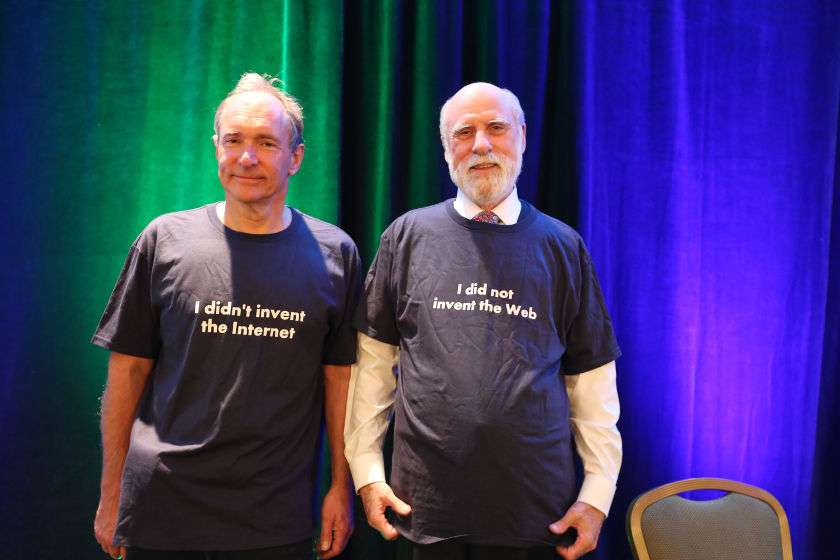
\includegraphics{src/img/0O4A8746-large.jpg}(1)

Donc, ce ne sont pas Gandalf (sans sa barbe) et Saruman mais bien Sir
Tim Berners-Lee et Vinton Cerf, responsables du (World Wide) Web et de
l'Internet.

\hypertarget{quest-ce-quinternet}{%
\subsection{\texorpdfstring{Qu'est-ce
qu'\href{https://www.youtube.com/watch?v=iDbyYGrswtg}{Internet}?}{Qu'est-ce qu'Internet?}}\label{quest-ce-quinternet}}

\begin{itemize}
\tightlist
\item
  un réseau IP
\end{itemize}

\hypertarget{quest-ce-que-le-world-wide-web}{%
\subsection{\texorpdfstring{Qu'est-ce que le
\href{http://line-mode.cern.ch/www/hypertext/WWW/TheProject.html}{World
Wide
Web}?}{Qu'est-ce que le World Wide Web?}}\label{quest-ce-que-le-world-wide-web}}

\begin{itemize}
\tightlist
\item
  \textbf{URI/URL}, des identifiants uniques
\item
  \textbf{HTML}, un langage de publication
\item
  \textbf{HTTP}, un protocole d'échange de texte (ou \emph{HyperText})
\end{itemize}

\hypertarget{pruxe9paratifs}{%
\section{Préparatifs}\label{pruxe9paratifs}}

\href{https://github.com/HE-Arc/php-intro-framework}{https://github.com/HE-Arc/php-intro-framework/}

\begin{otherlanguage}{english}

\begin{verbatim}
$ sudo systemctl start httpd
$ cd /var/www/html
$ git clone \
> https://github.com/\
> HE-Arc/php-intro-framework

$ cd php-intro-framework
$ open http://localhost/php-intro-framework
\end{verbatim}

\end{otherlanguage}

Les exemples suivant travaillent sur le code disponible dans le dépôt
\href{https://github.com/HE-Arc/php-intro-framework}{HE-Arc/php-intro-framework}.

\begin{otherlanguage}{english}

\begin{verbatim}

$ curl -v "http://he-arc.ch/?id=25"
> GET /?id=25 HTTP/1.1
> Host: he-arc.ch
>
< HTTP/1.1 200 OK
< Content-Type: text/html; charset=utf-8
<
\end{verbatim}

\end{otherlanguage}

\begin{otherlanguage}{english}

\begin{Shaded}
\begin{Highlighting}[]
\DataTypeTok{<!DOCTYPE }\NormalTok{html}\DataTypeTok{>}
\KeywordTok{<title>}\NormalTok{HE-Arc}\KeywordTok{</title>}
\KeywordTok{<p>}\NormalTok{Hello}
\end{Highlighting}
\end{Shaded}

\end{otherlanguage}

HTTP est un protocole texte plutôt simple, jugez plutôt:

Ce que nous voyons est une connexion TCP/IP au serveur
\begin{otherlanguage}{english}\texttt{he-arc.ch}\end{otherlanguage}. Une
fois la connexion établie, il envoie en texte ASCII les entêtes HTTP
puis deux retours à la ligne (ce qui correspond à une ligne vide). La
requête HTTP commencent toujours par la demande, ici
\begin{otherlanguage}{english}\texttt{GET\ /index.php?page=equipe\&id=25\ HTTP/1.1}\end{otherlanguage}
puis les entêtes, ici:
\begin{otherlanguage}{english}\texttt{Host:\ www.he-arc.ch}\end{otherlanguage}.
La réponse du serveur est du même type, le code de réponse
(\begin{otherlanguage}{english}\texttt{HTTP/1.1\ 200\ OK}\end{otherlanguage}),
les entêtes, une ligne vide puis le contenu.

La demande et les entêtes sont en US-ASCII mais le corps peut être
encodé autrement, ici c'est dit dans l'entête
\begin{otherlanguage}{english}\texttt{Content-Type:\ text/html;\ charset=utf-8}\end{otherlanguage}.

\hypertarget{fait-1}{%
\subsection{Fait \#1}\label{fait-1}}

PHP parle HTTP.

Le fichier
\begin{otherlanguage}{english}\texttt{index.php}\end{otherlanguage} est
le code PHP le plus simple qui soit. Simple au sens du niveau de
compréhension de PHP et d'une forme de complexité.

\begin{otherlanguage}{english}

\begin{Shaded}
\begin{Highlighting}[]
\KeywordTok{<?php} \CommentTok{// 00-base}

\CommentTok{// Lecture de la query string `page=<XX>&id=<YY>`.}
\KeywordTok{$page}\NormalTok{ = }\KeywordTok{$_GET}\OtherTok{[}\StringTok{"page"}\OtherTok{]} \OtherTok{??} \KeywordTok{null}\OtherTok{;}
\KeywordTok{$id}\NormalTok{ = }\DataTypeTok{(int)} \OtherTok{(}\KeywordTok{$_GET}\OtherTok{[}\StringTok{"id"}\OtherTok{]} \OtherTok{??} \DecValTok{0}\OtherTok{);}

\CommentTok{// Connexion à la base de données.}
\KeywordTok{$db}\NormalTok{ = }\KeywordTok{new} \KeywordTok{PDO}\OtherTok{(}\StringTok{"sqlite:../users.db"}\OtherTok{);}

\CommentTok{// Page HTML}
\KeywordTok{?>}
\NormalTok{<!}\KeywordTok{DOCTYPE}\NormalTok{ html>}
\NormalTok{<meta charset=utf}\DecValTok{-8}\NormalTok{>}
\NormalTok{<title>}\KeywordTok{HE}\NormalTok{-Arc</title>}
\NormalTok{<}\OtherTok{?}\NormalTok{php}
\CommentTok{// Contenu}
\KeywordTok{if} \OtherTok{(}\StringTok{"equipe"}\NormalTok{ === }\KeywordTok{$page}\OtherTok{):}
    \KeywordTok{$query}\NormalTok{ = }\KeywordTok{$db}\NormalTok{->query}\OtherTok{(}\StringTok{"SELECT * FROM `personnes` WHERE `id` = :id;"}\OtherTok{);}
    \KeywordTok{$query}\NormalTok{->execute}\OtherTok{(}\FunctionTok{compact}\OtherTok{(}\StringTok{'id'}\OtherTok{));}

    \KeywordTok{$personne}\NormalTok{ = }\KeywordTok{$query}\NormalTok{->fetch}\OtherTok{(}\KeywordTok{PDO}\NormalTok{::}\KeywordTok{FETCH_OBJ}\OtherTok{);}
\KeywordTok{?>}
\NormalTok{    <p><a href=}\StringTok{"<?php echo }\KeywordTok{$_SERVER}\StringTok{["}\KeywordTok{PHP_SELF}\StringTok{"] ?>"}\NormalTok{>retour</a>}
\NormalTok{    <h1>Équipe</h1>}
\NormalTok{    <h2>}
\NormalTok{        <}\OtherTok{?}\NormalTok{php }\KeywordTok{echo} \KeywordTok{$personne}\NormalTok{->prenom }\KeywordTok{?>}
\NormalTok{        <}\OtherTok{?}\NormalTok{php }\KeywordTok{echo} \KeywordTok{$personne}\NormalTok{->nom }\KeywordTok{?>}
\NormalTok{    </h2>}
\NormalTok{    <p>}
\NormalTok{        <img src=}\StringTok{"//www.gravatar.com/avatar/<?php}
\StringTok{            echo md5(strtolower(}\KeywordTok{$personne}\StringTok{->email));}
\StringTok{        ?>"}\NormalTok{ alt=}\StringTok{"avatar"}\NormalTok{>}
\NormalTok{<}\OtherTok{?}\NormalTok{php}
\KeywordTok{else}\OtherTok{:}
\KeywordTok{?>}
\NormalTok{    <h1>Accueil</h1>}
\NormalTok{    <ul>}
\NormalTok{        <li><a href=}\StringTok{"?page=equipe&amp;id=1"}\NormalTok{>Yoan Blanc</a>}
\NormalTok{        <li><a href=}\StringTok{"?page=equipe&amp;id=2"}\NormalTok{>Yoan Blanc</a>}
\NormalTok{    </ul>}
\NormalTok{<}\OtherTok{?}\NormalTok{php}
\KeywordTok{endif}
\end{Highlighting}
\end{Shaded}

\end{otherlanguage}

\hypertarget{fait-2}{%
\subsection{Fait \#2}\label{fait-2}}

PHP \textbf{est} un langage de template.

Pour preuve, il faut ouvrir une balise
\begin{otherlanguage}{english}\texttt{\textless{}?php}\end{otherlanguage}
pour commencer la partie code.

Avec la pratique, on a réalisé que de mélanger la logique métier et
celle d'affichage n'était pas optimale car difficile à lire et
maintenir.

\hypertarget{suxe9paration-muxe9tieraffichage}{%
\section{Séparation
métier/affichage}\label{suxe9paration-muxe9tieraffichage}}

\begin{otherlanguage}{english}

\begin{Shaded}
\begin{Highlighting}[]
\KeywordTok{<?php} \CommentTok{// 01-includes/index.php}

\CommentTok{// ...}

\KeywordTok{include} \StringTok{"templates/entete.html"}\OtherTok{;}

\KeywordTok{if} \OtherTok{(}\StringTok{"equipe"}\NormalTok{ === }\KeywordTok{$_GET}\OtherTok{[}\StringTok{"page"}\OtherTok{])}\NormalTok{ \{}
    \CommentTok{// SELECT FROM u WHERE id=$_GET["id"]}
    \CommentTok{// ...}
    \KeywordTok{include} \StringTok{"templates/equipe.html"}\OtherTok{;}
\NormalTok{\} }\KeywordTok{else}\NormalTok{ \{}
    \CommentTok{// ...}
    \KeywordTok{include} \StringTok{"templates/accueil.html"}\OtherTok{;}
\NormalTok{\}}
\end{Highlighting}
\end{Shaded}

\end{otherlanguage}


\includegraphics{src/img/meme10.jpg}

Quel est le problème avec cette solution?

(\href{https://raw.githubusercontent.com/cyrilmanuel/picbot/e6ff24a8bfd7ee9f0514a4fd8f49b1255ef26178/picbot/Images/meme10.jpg}{Source
de l'image})

\hypertarget{suxe9curituxe9-des-templates}{%
\section{Sécurité des templates}\label{suxe9curituxe9-des-templates}}

\begin{itemize}
\tightlist
\item
  \emph{Principle of Least Privilege} (
  \href{https://en.wikipedia.org/wiki/Principle_of_least_privilege}{polp}
  )
\item
  Intégration faite par un graphiste, société externe
\end{itemize}

Dans ce le cas présent rien ne nous empêche de mettre de la logique
métier dans nos fichiers de \emph{template}, car ils sont faits de PHP
eux aussi.

\begin{otherlanguage}{english}

\begin{Shaded}
\begin{Highlighting}[]
\NormalTok{\{# 02-twig/templates/collaborateur.html #\}}
\NormalTok{\{%- extends "base.html" -%\}}

\NormalTok{\{% block corps -%\}}
\KeywordTok{<p><a}\OtherTok{ href=}\StringTok{"?"}\KeywordTok{>}\NormalTok{retour}\KeywordTok{</a>}
\KeywordTok{<h1>}\NormalTok{Équipe}\KeywordTok{</h1>}
\KeywordTok{<h2>}
\NormalTok{  \{\{- personne.prenom -\}\}}
\NormalTok{  \{\{ personne.nom -\}\}}
\KeywordTok{</h2>}
\KeywordTok{<p><img}
\OtherTok{  src=}\StringTok{"//www.gravatar.com/avatar/}
\StringTok{  \{\{- personne.email | strtolower | md5 \}\}"}
\OtherTok{  alt=}\StringTok{"avatar"}\KeywordTok{>}
\NormalTok{\{% endblock -%\}}
\end{Highlighting}
\end{Shaded}

\end{otherlanguage}

La page est réalisée avec \href{http://twig.sensiolabs.org/}{Twig}
\textless{}2.0. À partir de la version 2.0, il faut utiliser un
\emph{autoloader} externe, comme celui de composer (voir ci-dessous).

Le code est un poil plus propre du côté de nos \emph{templates} qui ne
peuvent plus exécuter de PHP sauf ce qu'on leur autorise, ici
\begin{otherlanguage}{english}\texttt{md5}\end{otherlanguage} et
\begin{otherlanguage}{english}\texttt{strtolower}\end{otherlanguage}.
Voir
\href{02-twig/index.php}{\begin{otherlanguage}{english}\texttt{02-twig/index.php}\end{otherlanguage}}.

\begin{otherlanguage}{english}

\begin{Shaded}
\begin{Highlighting}[]
\KeywordTok{<?php} \CommentTok{// 02-twig}

\KeywordTok{require_once} \StringTok{'Twig/lib/Twig/Autoloader.php'}\OtherTok{;}
\NormalTok{Twig_Autoloader::register}\OtherTok{();}

\CommentTok{// ...}

\CommentTok{// Configuration de Twig}
\KeywordTok{$loader}\NormalTok{ = }\KeywordTok{new}\NormalTok{ Twig_Loader_FileSystem}\OtherTok{(}\StringTok{"templates"}\OtherTok{);}
\KeywordTok{$twig}\NormalTok{ = }\KeywordTok{new}\NormalTok{ Twig_Environment}\OtherTok{(}\KeywordTok{$loader}\OtherTok{);}

\CommentTok{// Ajout des filtres md5 et strtolower qui sont les fonctions PHP du même nom.}
\KeywordTok{$twig}\NormalTok{->addFilter}\OtherTok{(}\KeywordTok{new}\NormalTok{ Twig_SimpleFilter}\OtherTok{(}\StringTok{'strtolower'}\OtherTok{,} \StringTok{'strtolower'}\OtherTok{));}
\KeywordTok{$twig}\NormalTok{->addFilter}\OtherTok{(}\KeywordTok{new}\NormalTok{ Twig_SimpleFilter}\OtherTok{(}\StringTok{'md5'}\OtherTok{,} \StringTok{'md5'}\OtherTok{));}

\CommentTok{// variable globale}
\KeywordTok{$titre}\NormalTok{ = }\StringTok{"HE-Arc"}\OtherTok{;}

\CommentTok{// Contenu}
\KeywordTok{if} \OtherTok{(}\StringTok{"equipe"}\NormalTok{ === }\KeywordTok{$page}\OtherTok{)}\NormalTok{ \{}
    \CommentTok{// ...}
    \KeywordTok{$personne}\NormalTok{ = }\CommentTok{// ...}

    \KeywordTok{echo} \KeywordTok{$twig}\NormalTok{->render}\OtherTok{(}\StringTok{"equipe.html"}\OtherTok{,} \FunctionTok{compact}\OtherTok{(}\StringTok{"titre"}\OtherTok{,} \StringTok{"personne"}\OtherTok{));}
\NormalTok{\} }\KeywordTok{else}\NormalTok{ \{}
    \KeywordTok{$personnes}\NormalTok{ = }\CommentTok{// ...}

    \KeywordTok{echo} \KeywordTok{$twig}\NormalTok{->render}\OtherTok{(}\StringTok{"accueil.html"}\OtherTok{,} \FunctionTok{compact}\OtherTok{(}\StringTok{"titre"}\OtherTok{,} \StringTok{"personnes"}\OtherTok{));}
\NormalTok{\}}
\end{Highlighting}
\end{Shaded}

\end{otherlanguage}

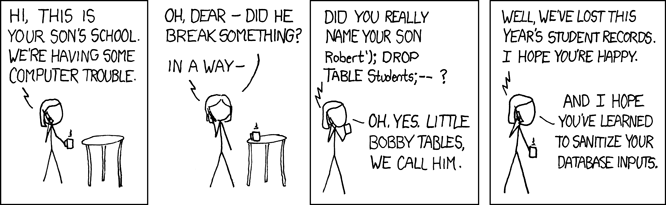
\includegraphics{src/img/exploits_of_a_mom.png} Problème d'injection
SQL.

Effectuer des requêtes MySQL à la main ou devoir connaitre tous les
champs crée beaucoup de redondance et de failles de sécurité
potentielles.

Une solution est d'ajouter une couche d'abstraction qui va cacher la
structure réelle de notre base de données et offrir une interface
orientée objet. Un \emph{Object-Relational Mapping} ou ORM(3) dans le
jargon.

\begin{otherlanguage}{english}

\begin{Shaded}
\begin{Highlighting}[]

\KeywordTok{<?php}
\CommentTok{// Ne dites plus}
\KeywordTok{$query}\NormalTok{ = }\KeywordTok{$db}\NormalTok{->query}\OtherTok{(}
  \StringTok{"SELECT * FROM `personnes` "}\NormalTok{.}
  \StringTok{"WHERE `id` = :id;"}
\OtherTok{);}
\KeywordTok{$query}\NormalTok{->execute}\OtherTok{(}\FunctionTok{compact}\OtherTok{(}\StringTok{'id'}\OtherTok{));}
\KeywordTok{$personne}\NormalTok{ = }\KeywordTok{$query}\NormalTok{->fetch}\OtherTok{(}\KeywordTok{PDO}\NormalTok{::}\KeywordTok{FETCH_OBJ}\OtherTok{);}

\CommentTok{// Mais dites plutôt}

\CommentTok{//  RedBean}
\KeywordTok{$personne}\NormalTok{ = }\KeywordTok{R}\NormalTok{::load}\OtherTok{(}\StringTok{'personnes'}\OtherTok{,} \KeywordTok{$id}\OtherTok{);}
\CommentTok{// ou Doctrine}
\KeywordTok{$personne}\NormalTok{ = }\KeywordTok{$om}\NormalTok{->find}\OtherTok{(}\StringTok{'Personne'}\OtherTok{,} \KeywordTok{$id}\OtherTok{);}
\end{Highlighting}
\end{Shaded}

\end{otherlanguage}

\hypertarget{object-relational-mapping}{%
\section{\texorpdfstring{\emph{Object-Relational
Mapping}}{Object-Relational Mapping}}\label{object-relational-mapping}}

\begin{itemize}
\tightlist
\item
  \href{http://www.redbeanphp.com/}{RedBean}
\item
  \href{http://www.doctrine-project.org/}{Doctrine} (ORM, ODM)
\item
  \href{http://laravel.com/docs/master/eloquent}{Eloquent ORM}
\item
  \href{https://en.wikipedia.org/wiki/List_of_object-relational_mapping_software\#PHP}{etc.}
\end{itemize}

Une bibliothèque qui va créer ce lien entre les mondes objet et
relationnel ou document (généralement MongoDB). Il en existe toute une
foule.

\begin{otherlanguage}{english}

\begin{Shaded}
\begin{Highlighting}[]
\KeywordTok{<?php} \CommentTok{// 03-redbean/index.php}
\KeywordTok{require} \StringTok{'RedBean/rb.php'}\OtherTok{;}
\KeywordTok{R}\NormalTok{::setup}\OtherTok{(}\StringTok{"sqlite:../users.db"}\OtherTok{);}
\CommentTok{// ...}
\KeywordTok{if} \OtherTok{(}\StringTok{"equipe"}\NormalTok{ === }\KeywordTok{$page}\OtherTok{)}\NormalTok{ \{}
    \KeywordTok{$personne}\NormalTok{ = }\KeywordTok{R}\NormalTok{::load}\OtherTok{(}\StringTok{"personnes"}\OtherTok{,} \KeywordTok{$id}\OtherTok{);}
    \KeywordTok{echo} \KeywordTok{$twig}\NormalTok{->render}\OtherTok{(}
        \StringTok{"equipe.html"}\OtherTok{,}
        \FunctionTok{compact}\OtherTok{(}\StringTok{"titre"}\OtherTok{,} \StringTok{"personne"}\OtherTok{)}
    \OtherTok{);}
\NormalTok{\} }\KeywordTok{else}\NormalTok{ \{}
    \KeywordTok{$personnes}\NormalTok{ = }\KeywordTok{R}\NormalTok{::find}\OtherTok{(}\StringTok{"personnes"}\OtherTok{);}
    \KeywordTok{echo} \KeywordTok{$twig}\NormalTok{->render}\OtherTok{(}
        \StringTok{"accueil.html"}\OtherTok{,}
        \FunctionTok{compact}\OtherTok{(}\StringTok{"titre"}\OtherTok{,} \StringTok{"personnes"}\OtherTok{)}
    \OtherTok{);}
\NormalTok{\}}
\end{Highlighting}
\end{Shaded}

\end{otherlanguage}

\hypertarget{uri-as-ui}{%
\section{URI as UI}\label{uri-as-ui}}

Pensez à Wikipedia.

Les adresses des pages font partie de l'expérience utilisateur. Un
utilisateur doit être capable d'imaginer le contenu de la page en lisant
l'URI. Certainement, ce que vous faites avant de cliquer sur un lien.

\hypertarget{comment-humaniser}{%
\subsection{Comment humaniser ?}\label{comment-humaniser}}

\begin{otherlanguage}{english}

\begin{verbatim}
  /index.php?page=equipe&id=42
\end{verbatim}

\end{otherlanguage}

La personne avec l'identifiant
\begin{otherlanguage}{english}\texttt{42}\end{otherlanguage} aura
également un \emph{slug} unique créé à partir de son nom, ici
\begin{otherlanguage}{english}\texttt{jean-bon}\end{otherlanguage}.

La solution à notre problème est de demander au serveur web de réécrire
les URL pour nous.

\hypertarget{ruxe9uxe9criture-durl}{%
\subsection{Réécriture d'URL}\label{ruxe9uxe9criture-durl}}

\begin{otherlanguage}{english}

\begin{Shaded}
\begin{Highlighting}[]
\CommentTok{# 04-routes/.htaccess}

\CommentTok{# mod_rewrite}
\ExtensionTok{RewriteEngine}\CharTok{ }\KeywordTok{on}
\NormalTok{RewriteBase}\StringTok{ /php-intro-framework/04-routes/}

\NormalTok{RewriteCond}\StringTok{ %\{REQUEST_FILENAME\} !-f}
\NormalTok{RewriteCond}\StringTok{ %\{REQUEST_FILENAME\} !-d}
\NormalTok{RewriteRule}\StringTok{ ^(.*)$ index.php/$1 [L,QSA]}
\end{Highlighting}
\end{Shaded}

\end{otherlanguage}

Apache le fait via
\href{https://httpd.apache.org/docs/current/mod/mod_rewrite.html}{\begin{otherlanguage}{english}\texttt{mod\_rewrite}\end{otherlanguage}}
et Nginx
\href{http://nginx.org/en/docs/http/ngx_http_core_module.html\#try_files}{\begin{otherlanguage}{english}\texttt{try\_files}\end{otherlanguage}}.

\begin{otherlanguage}{english}

\begin{Shaded}
\begin{Highlighting}[]

\CommentTok{// 04-routes/index.php}

\KeywordTok{$uri}\NormalTok{ = }\KeywordTok{$_SERVER}\OtherTok{[}\StringTok{'REQUEST_URI'}\OtherTok{],}
\KeywordTok{$matches}\NormalTok{ = }\OtherTok{[];}

\FunctionTok{preg_match}\OtherTok{(}
    \StringTok{"#^/(?P<page>[^/]+)/(?P<slug>[^/]+)/?#"}\OtherTok{,}
    \KeywordTok{$uri}\OtherTok{,}
    \KeywordTok{$matches}
\OtherTok{)} \KeywordTok{or} \KeywordTok{die}\OtherTok{(}\StringTok{'Arrrrrgh'}\OtherTok{);}

\KeywordTok{echo} \FunctionTok{call_user_func_array}\OtherTok{(}
    \KeywordTok{$matches}\OtherTok{[}\StringTok{'page'}\OtherTok{],}
    \OtherTok{[}\KeywordTok{$matches}\OtherTok{[}\StringTok{'slug'}\OtherTok{]]}
\OtherTok{);}
\end{Highlighting}
\end{Shaded}

\end{otherlanguage}

Le code complet va nettoyer l'URI et définir les fonction correspondant
aux pages possibles.

\hypertarget{routing}{%
\section{\texorpdfstring{\emph{Routing}}{Routing}}\label{routing}}

Lien entre les adresses (URI) et des actions dans le code.

a.k.a. the \emph{Front Controller}.

En pratique, les actions ne sont pas des fonctions mises à plat mais
sont encapsulées dans une classe qu'on nomme un contrôleur. Faire ainsi
permet de regrouper logiquement les fonctions et éviter d'utiliser
d'affreux éléments tel que
\begin{otherlanguage}{english}\texttt{global}\end{otherlanguage}.

\hypertarget{moduxe8le---vue---contruxf4leur}{%
\section{Modèle - Vue -
Contrôleur}\label{moduxe8le---vue---contruxf4leur}}

\begin{itemize}
\tightlist
\item
  Modèle: l'ORM qui s'occupe de notre base de données
\item
  Vue: les templates qui affiche les données
\item
  Contrôleur: une classe qui définit quoi faire en fonction des entrées
  utilisateur (URI, formulaire, etc.)
\end{itemize}

\emph{MVC}(4) vient des applications bureau et ne représente pas
toujours le fonctionnement dans le monde du web. Par exemple, Django, un
framework Python, se décrit comme étant \emph{Modèle - Template -
Vue}(5).

Les frameworks web en PHP (ou d'autres langages) reposent
majoritairement sur ce paradigme.

\hypertarget{composer}{%
\section{\texorpdfstring{\emph{Composer}}{Composer}}\label{composer}}

Gestionnaire de paquets pour PHP:
\href{http://getcomposer.org/}{getcomposer.org}

Maintenir notre répertoire de \emph{vendor} ainsi que les
\begin{otherlanguage}{english}\texttt{require}\end{otherlanguage} est
peu pratique. Voici qu'entre en scène
\href{http://getcomposer.org/}{Composer}, le gestionnaire de paquet pour
PHP. \href{https://packagist.org/}{Packagist} est le dépôt en ligne de
paquets public et utilisé par défaut.

\hypertarget{composer.json}{%
\subsection{composer.json}\label{composer.json}}

\begin{otherlanguage}{english}

\begin{Shaded}
\begin{Highlighting}[]
\FunctionTok{\{}
    \DataTypeTok{"require"}\FunctionTok{:} \FunctionTok{\{}
        \DataTypeTok{"twig/twig"}\FunctionTok{:} \StringTok{"^2.0"}\FunctionTok{,}
        \DataTypeTok{"gabordemooij/redbean"}\FunctionTok{:} \StringTok{"^4.3"}\FunctionTok{,}
    \FunctionTok{\}}
\FunctionTok{\}}
\end{Highlighting}
\end{Shaded}

\end{otherlanguage}

Nos dépendances sont ainsi matérialisées dans le projet et peuvent être
installée, ou mises à jour simplement.

En principe les numéros de version respectent le
\href{http://semver.org/lang/fr/}{SemVer} (\emph{Semantic Versioning})
et les différents signes permettent de sélection une ou plusieurs
versions (voir {[}Version and
constraints{]}{[}https://getcomposer.org/doc/articles/versions.md{]}).

\begin{otherlanguage}{english}

\begin{verbatim}


$ composer install
\end{verbatim}

\end{otherlanguage}

puis

\begin{otherlanguage}{english}

\begin{Shaded}
\begin{Highlighting}[]
\KeywordTok{<?php} \CommentTok{// 05-composer/index.php}

\KeywordTok{require} \StringTok{'vendor/autoload.php'}\OtherTok{;}

\KeywordTok{use}\NormalTok{ RedBeanPHP\textbackslash{}Facade }\KeywordTok{as} \KeywordTok{R}\OtherTok{;}
\end{Highlighting}
\end{Shaded}

\end{otherlanguage}

Enfin, nous pouvons réduire le nombre de
\begin{otherlanguage}{english}\texttt{require}\end{otherlanguage} et
\begin{otherlanguage}{english}\texttt{include}\end{otherlanguage} à un
seul, en laissant soin à l'\emph{auto-loader} de charger le bon fichier
à la demande. Tout ceci est spécifié dans
\href{http://www.php-fig.org/psr/psr-4/}{PSR-4}. Ainsi, les définitions
de Twig sont présentes et il nous suffit d'obtenir la classe
\begin{otherlanguage}{english}\texttt{R}\end{otherlanguage} depuis
\href{http://www.redbeanphp.com/}{RedBean}.

\hypertarget{front-controller}{%
\section{\texorpdfstring{\emph{Front-Controller}}{Front-Controller}}\label{front-controller}}

Utilisation de \href{https://github.com/nikic/FastRoute}{FastRoute}
(voir
\href{https://github.com/HE-Arc/php-intro-framework/blob/master/06-fastroute/index.php}{06-fastroute/index.php}).

\begin{otherlanguage}{english}

\begin{verbatim}
$ composer require nikic/fast-route
\end{verbatim}

\end{otherlanguage}

\begin{otherlanguage}{english}\texttt{FastRoute}\end{otherlanguage}
repose sur un système proche de celui que nous avons utilisé jusqu'ici.
D'autres systèmes, tels que
\begin{otherlanguage}{english}\texttt{Aura.Router}\end{otherlanguage}
pour ne citer que lui, reposent sur la spécification
\href{http://www.php-fig.org/psr/psr-7/}{PSR-7}. Cette dernière décrit
l'interface objet d'un message HTTP, tant au niveau de la requête que de
la réponse.

Si ça ajoute, une bonne couche de complexité, l'énorme avantage offert
par cette idée là est de déléguer le rendu d'une page, ni
\begin{otherlanguage}{english}\texttt{echo}\end{otherlanguage}, ni
\begin{otherlanguage}{english}\texttt{header}\end{otherlanguage}, Donc
il est envisageable de pouvoir tester (au sens de test unitaire), notre
\emph{FrontController}.

D'autre part, le
\begin{otherlanguage}{english}\texttt{call\_user\_func\_array}\end{otherlanguage}
d'avant n'était pas très solide,

\begin{otherlanguage}{english}

\begin{Shaded}
\begin{Highlighting}[]

\KeywordTok{<?php} \CommentTok{// 06-fastroute/index.php}
\CommentTok{// ...}
\KeywordTok{use} \KeywordTok{function}\NormalTok{ FastRoute\textbackslash{}simpleDispatcher}\OtherTok{;}
\KeywordTok{use}\NormalTok{ FastRouter\textbackslash{}Dispatcher}\OtherTok{;}

\KeywordTok{$dispatcher}\NormalTok{ = simpleDispatcher}\OtherTok{(}\KeywordTok{function}\OtherTok{(}\KeywordTok{$r}\OtherTok{)}
\NormalTok{\{}
    \KeywordTok{$r}\NormalTok{->addRoute}\OtherTok{(}\StringTok{'GET'}\OtherTok{,} \StringTok{'/'}\OtherTok{,} \StringTok{'accueil'}\OtherTok{);}

    \KeywordTok{$r}\NormalTok{->addRoute}\OtherTok{(}
        \StringTok{'GET'}\OtherTok{,}
        \StringTok{'/equipe/\{slug\}'}\OtherTok{,}
        \StringTok{'equipe'}
    \OtherTok{);}
\NormalTok{\}}\OtherTok{);}
\end{Highlighting}
\end{Shaded}

\end{otherlanguage}

\begin{otherlanguage}{english}

\begin{Shaded}
\begin{Highlighting}[]
\KeywordTok{<?php} \CommentTok{// 06-fastroute/index.php (suite)}

\KeywordTok{$httpMethod}\NormalTok{ = }\KeywordTok{$_SERVER}\OtherTok{[}\StringTok{"REQUEST_METHOD"}\OtherTok{];}
\KeywordTok{$uri}\NormalTok{ = }\KeywordTok{$_SERVER}\OtherTok{[}\StringTok{"REQUEST_URI"}\OtherTok{];}

\CommentTok{// nettoyage de $uri}
\CommentTok{// - prefix}
\CommentTok{// - query string}
\CommentTok{// - caractères spéciaux (e.g. %20)}

\KeywordTok{$routeInfo}\NormalTok{ = }\KeywordTok{$dispatcher}\NormalTok{->dispatch}\OtherTok{(}
    \KeywordTok{$httpMethod}\OtherTok{,}
    \KeywordTok{$uri}
\OtherTok{);}
\end{Highlighting}
\end{Shaded}

\end{otherlanguage}

\begin{otherlanguage}{english}

\begin{Shaded}
\begin{Highlighting}[]
\KeywordTok{<?php} \CommentTok{// 06-fastroute (suite)}

\KeywordTok{switch}\OtherTok{(}\KeywordTok{$routeInfo}\OtherTok{[}\DecValTok{0}\OtherTok{])}\NormalTok{ \{}
    \KeywordTok{case }\NormalTok{Dispatcher::}\KeywordTok{NOT_FOUND}\OtherTok{:}
    \KeywordTok{case }\NormalTok{Dispatcher::}\KeywordTok{METHOD_NOT_ALLOWED}\OtherTok{:}
        \CommentTok{/* ... */}\KeywordTok{break}\OtherTok{;}
    \KeywordTok{case }\NormalTok{Dispatcher::}\KeywordTok{FOUND}\OtherTok{:}
        \KeywordTok{try}\NormalTok{ \{}
            \KeywordTok{echo} \FunctionTok{call_user_func_array}\OtherTok{(}
                \KeywordTok{$routeInfo}\OtherTok{[}\DecValTok{1}\OtherTok{],}
                \KeywordTok{$routeInfo}\OtherTok{[}\DecValTok{2}\OtherTok{]}
            \OtherTok{);}
\NormalTok{        \} }\KeywordTok{catch} \OtherTok{(}\KeywordTok{Exception} \KeywordTok{$e}\OtherTok{)}\NormalTok{\{}
            \KeywordTok{echo}\NormalTok{ server_error}\OtherTok{(}\KeywordTok{$e}\OtherTok{);}
\NormalTok{        \}}
        \KeywordTok{break}\OtherTok{;}
\NormalTok{\}}
\end{Highlighting}
\end{Shaded}

\end{otherlanguage}

\hypertarget{framework-php}{%
\section{\texorpdfstring{\emph{Framework
PHP}}{Framework PHP}}\label{framework-php}}

Une collection de bibliothèques avec un peu de glue.

Un framework web vous propose une structure de base pour construire
selon une méthode jugée bonne par ses concepteurs. Il est possible de
remplacer un composant par un autre, par le sien. Et même de créer sa
\emph{glue} ou même ses outils propres.

\hypertarget{liens-avec-laravel}{%
\subsection{Liens avec Laravel}\label{liens-avec-laravel}}

\begin{itemize}
\tightlist
\item
  Modèle MVC
\item
  Templates utilisant \emph{blade}.
\item
  ORM nommé \emph{Eloquent}.
\item
  \emph{Front-Controller}
  (\begin{otherlanguage}{english}\texttt{Illuminate\textbackslash{}Routing}\end{otherlanguage})
\item
  Bibliothèques \ldots{}
  (\begin{otherlanguage}{english}\texttt{Illuminate\textbackslash{}*}\end{otherlanguage})
\item
  \href{http://getcomposer.org/}{Composer}
\end{itemize}

Je vous invite à aller lire le code généré pour vous par Laravel. Vous
allez retrouver ces éléments. Symfony, CakePHP, etc. auront les mêmes
idées.

\hypertarget{exercice}{%
\subsection{Exercice}\label{exercice}}

\begin{itemize}
\tightlist
\item
  Refaites les différentes étapes à partir de
  \begin{otherlanguage}{english}\texttt{00-base}\end{otherlanguage}.
\item
  Tel quel ou en utilisant d'autres bibliothèques :
  \href{https://github.com/smarty-php/smarty}{Smarty},
  \href{http://docs.doctrine-project.org/en/latest/tutorials/getting-started.html}{Doctrine},
  \href{https://github.com/auraphp/Aura.Router}{Aura.Router}
\end{itemize}

\hypertarget{fin}{%
\section{Fin}\label{fin}}

Questions?

\begin{otherlanguage}{english}

\end{otherlanguage}

\begin{otherlanguage}{english}

\end{otherlanguage}

\begin{otherlanguage}{english}

\end{otherlanguage}

\hypertarget{sources}{%
\section*{Sources}\label{sources}}
\addcontentsline{toc}{section}{Sources}

\hypertarget{refs}{}
\leavevmode\hypertarget{ref-w3c:20}{}%
1. W3C. W3C 20 Anniversary Symposium. {[}en~ligne{]}. 2014.
{[}Consulté~le~7~février~2017{]}. Disponible à l'adresse~:
\url{https://www.w3.org/20/Overview.html}

\leavevmode\hypertarget{ref-xkcd:327}{}%
2. MUNROE, Randall. Exploits of a mom. {[}en~ligne{]}. 2007.
{[}Consulté~le~7~février~2017{]}. Disponible à l'adresse~:
\url{https://xkcd.com/327/}

\leavevmode\hypertarget{ref-wiki:orm}{}%
3. WIKIPEDIA. \emph{Mapping objet-relationnel} {[}en~ligne{]}.
{[}Consulté~le~7~février~2017{]}. Disponible à l'adresse~:
\url{https://fr.wikipedia.org/wiki/Mapping_objet-relationnel}

\leavevmode\hypertarget{ref-wiki:mvc}{}%
4. WIKIPEDIA. Modèle-Vue-Contrôleur. {[}en~ligne{]}.
{[}Consulté~le~7~février~2017{]}. Disponible à l'adresse~:
\url{https://fr.wikipedia.org/wiki/Modèle-vue-contrôleur}

\leavevmode\hypertarget{ref-django:mtv}{}%
5. DJANGO PROJECT. Django appears to be a MVC framework, but you call
the Controller the «~view~», and the View the «~template~». How come you
don't use the standard names? \emph{FAQ: General} {[}en~ligne{]}.
{[}Consulté~le~7~février~2017{]}. Disponible à l'adresse~:
\url{https://docs.djangoproject.com/en/1.11/faq/general/\#django-appears-to-be-a-mvc-framework-but-you-call-the-controller-the-view-and-the-view-the-template-how-come-you-don-t-use-the-standard-names}
